\documentclass[12pt,hidelinks]{article}
\ifx\pdfoutput\undefined 
\usepackage[dvips]{graphicx}
\else
\usepackage[pdftex]{graphicx} 
\usepackage{type1cm} \fi
\usepackage{a4}
\usepackage{lastpage}
\usepackage{graphicx,hyperref,amsmath,bm,url}
\usepackage[numbers]{natbib}
\usepackage{microtype,todonotes}
\usepackage{a4}
\usepackage[compact,small]{titlesec}
\usepackage[utf8]{inputenc}
\clubpenalty = 10000
\widowpenalty = 10000
\usepackage[T1]{fontenc}
\graphicspath{ {../Billeder/} }
\usepackage{tikz}
\usetikzlibrary{calc}
\usetikzlibrary{shapes}
\usepackage[labelfont=bf]{caption}
\renewcommand{\figurename}{\textbf{Figur}}
\renewcommand{\contentsname}{Indholdfortegnelse}
\renewcommand{\refname}{Referencer}

\makeatletter
\newdimen\@myBoxHeight%
\newdimen\@myBoxDepth%
\newdimen\@myBoxWidth%
\newdimen\@myBoxSize%
\newcommand{\SquareBox}[2][]{%
    \settoheight{\@myBoxHeight}{#2}% Record height of box
    \settodepth{\@myBoxDepth}{#2}% Record depth of box
    \settowidth{\@myBoxWidth}{#2}% Record width of box
    \pgfmathsetlength{\@myBoxSize}{max(\@myBoxWidth,(\@myBoxHeight+\@myBoxDepth))}%
    \tikz \node [shape=rectangle, shape aspect=1,draw=red,inner sep=2\pgflinewidth, minimum size=\@myBoxSize,#1] {#2};%
}%
\makeatother
\newcommand*{\captionsource}[2]{%
  \caption[{#1}]{%
    #1%
    \\\hspace{\linewidth}%
    \textbf{Kilde:} #2%
  }%
}
\usepackage{lscape}
\usepackage[ddmmyyyy]{datetime}
\newcommand{\school}{Kærbyskolen }
\setcounter{secnumdepth}{4}

\begin{document}
	\sloppy

	\begin{titlepage}
	\begin{nopagebreak}
	{\small\samepage 
	\hfill\begin{tabular}{r}
	\parbox{6cm}{  \raisebox{11mm}{
\includegraphics[height=1.3cm]{aaulogo}}
	\hfill \parbox{4.9cm}{\begin{tabular}{l}
	{\sf\small \textbf{Det Teknisk-Naturvidenskabelige Basis{\aa}r }}\\
	{\sf\small  \textbf{Datalogi}} \\
	{\sf\small Strandvejen 12-14} \\
	{\sf\small Telefon 96 35 97 31} \\
	{\sf\small Fax 98 13 63 93} \\
	{\sf\small http://tnb.aau.dk}
	\end{tabular}}}
	\\
	\end{tabular}

	\begin{tabular}{cc}
	\parbox{7cm}{
	\begin{description}

	\item {\bf Titel: \\Titel} 
	  
	\item {\bf Tema: \\Skemalægning i folkeskoler ved hjælp af generiske algoritmer} 

	\end{description}

	\parbox{7cm}{

	\begin{description}
	\item {\bf Projektperiode: \\P1}
		\\
	  \hspace{3cm}
	\item {\bf Gruppe: \\B2-2}
	\\
	  \hspace{3cm}
	\item {\bf Deltagere: \\ Frederik Kær\\Jacob Svenningsen\\ Mathias Jakobsen\\Theresa Krogh Walker\\  Søren Madsen \\Morten Hansen}\\
	  \hspace{2cm}
	\item {\bf Vejledere: \\Claus Skaaning og Søren Kerndrup}\\
	\end{description}
	}
	\begin{description}
	\item {\bf Antal sider: \\\pageref{LastPage}} 
	%\item {\bf Bilagsantal og --art:} ??
	\item {\bf Afsluttet den \today} 
	\end{description}
	\vfill } &
	\parbox{7cm}{
	  \vspace{.15cm}
	  \hfill 
	  \begin{tabular}{l}
	  {\bf Synopsis:}\bigskip \\
	  \fbox{
	    \parbox{6.5cm}{\bigskip
	     {\vfill{\small I dette projekt analyseres og belyses emnet skemalægning i folkeskoler samt de arbejdsmæssige udfordringer, det at lægge skemaer giver. Der redegøres for forskellige typer af skemadannelse og for de valg, der må træffes, når der lægges skemaer.
	     \bigskip}}
	     }}
	   \end{tabular}}
	\end{tabular}}
	\\ \\
	%\noindent{\footnotesize\emph{Rapportens indhold er frit tilgængeligt, men offentliggørelse (med kildeangivelse) må kun ske efter aftale med forfatterne.}}
	\end{nopagebreak}
	\end{titlepage}

	
	\addtocounter{page}{1}

	\newpage
	\tableofcontents
	\newpage
	\section{Indledning}
	
I vores problemafgrænsning ønsker vi at indsnævre det problem, som tages med fra problemanalysen og finde frem til de fokusområder, som vi finder vigtigst inden for skemalægning i folkeskoler og ønsker at tage udgangspunkt i under problemløsningen. Prolemafgrænsningen skulle altså gerne hjælpe med at finde frem til en god problemformulering. Det vil i afsnittet altså blive beskrevet, hvilke fokusområder der til- og fravælges.

For at sikre et projekt, som har relevans i vores tid og for vores specifikke case, tages der udgangspunkt i vores case, Kærbyskolen, og kun \school da vi grundet tidspres, ikke har tid til at inkludere flere cases samtidig med at sikre vores løsning er kompatibel under begge skolers skemalægningsprocedure og publiceringen af disse.

\subsection*{Pædagogisk læring}
På Kærbyskolen har skemaer, som tager deres udgangspunkt i pædagogisk læring og elevtrivsel, i år været højt prioriteret. Dette kom til udtryk under interviewet med skolen, hvor det blev beskrevet, at pædagogiske overvejelser i forhold til skemalægning blev diskuteret meget og var noget, som nuværende løsninger i følge skolen ikke forholder sig nok til. Vi ønsker derfor at lægge fokus på skemalægning med vægt på pædagogisk overvejelser.

\subsubsection*{Brugergrænseflade}
Brugergrænseflade fravælges som fokusområde og dette gøres hovedsageligt grundet projektets omfang og tidsbegrænsning. Dette betyder dog ikke, at brugervenlighed glemmes helt. Kærbyskolen lagde under det foretagede interview vægt på, at programmer skal være nemme at bruge, og at det er vigtigt, at programmet løbende giver brugeren en status. Dette ønsker vi så at tage hensyn til i så stort et omfang, som muligt.

\subsubsection*{Andre afgrænsninger}
I forbindelse med overvejelser omkring projektets omfang og de opstillede tidsbegrænsninger, som vi må forholde os til, har vi desuden måtte gøre os nogle andre fravalg af fokuspunkter. Dette er valg som vi føler er nødvendige for, at projektet realistisk kan gennemføres i tide og samtidig ikke rammer den egentlige kvalitet af problemløsningen eller programfunktionalitet, men blot gør det endelige program lidt mindre.

Vi har med valget af Kærbyskolen som case fravalgt at tage højde for valgfag, da skolen kun går til 6. klasse, hvor disse endnu ikke findes. 

Vores case, Kærbyskolen, er en meget lille skole og derfor har de ikke mulighed for at have alle fagene på skolens grund. Kærbyskolen er nødt til at arbejde sammen med andre parter for at opfylde kraverne om idræts- og hjemkundsskabsfaciliteter. Vi har dog valgt, at fokuset ikke skal være lagt på lokalerne, men på pædagogisk læring og brugerflade.

Vi fokuserer på skemalægning på Kærbyskolen, men ønsker ikke at tage højde for skolens såkaldte J-klasser for autismediagnostiserede elever, da der dannes skemaer efter elevens individuelle behov. Derfor vil vi fokusere på at lægge skema til klasserne 0 til 6.

%\subsubsection*{Valgfag}
%Vi har fravalgt valgfag, som et fokusemne, da vi har valgt at arbejde ud fra en case, hvor skolen i dette tilfælde går op til 6. klasse, hvor de ikke har valgfag.

%\subsubsection*{Lokaler}
%Vores case, Kærbyskolen, er en meget lille skole og derfor  har de ikke mulighed for at have alle fagene på skolensgrund. Kærbyskolen er nødt til at arbejde sammen med andre parter for at opfylde kraverne om idræts og hjemkundsskabs faciliteter. Vi har dog valgt, at fokuset ikke skal være lagt på lokalerne, men på pædagogisk læring og brugerflade.

%Vi fokuserer på skemalægning på Kærbyskolen, men ønsker ikke at tage højde for skolens såkaldte J-klasser for autismediagnostiserede elever, da der dannes skemaer efter elevens individuelle behov. Derfor vil vi fokusere på at lægge skema til klasserne 0 til 6.

	\section{Problemanalyse}
	\subsection{Lovgivning og regler for skemalægning}
\label{Lovgivning og regler}
I driften af en folkeskole er planlægning et utroligt vigtigt redskab i opnåelsen af en velfungerende og læringsrig hverdag for såvel lærere som elever, sekretærer og andet personale. Planlægning er altafgørende og et godt skema ligeså. I folkeskolen er hverdagen som hovedregel baseret på de ugeskemaer, der som minimum inden starten af hvert skoleår udarbejdes af skolen og sidenhen følges nøje. Fungerer dette skema ikke, er der en stor risiko for, at hverdagen ej heller fungerer og undervisningsniveauet rammes af det.

Dette er en af grundene til, at der hvert år lægges utroligt mange timer i skemalægning på hver eneste folkeskole i landet og oftest er der tale om et større team, som må samle sig om opgaven. Hvad der gør det så utroligt svært at lægge et velfungerende skema er den nærmeste uendelige liste af lovgivninger, regler, krav og bindinger som de skemalæggende teams er nødsagede til at tage hensyn til.  Der stilles krav til skolen af det danske undervisningsministerium i form af bl.a. de nationale Fælles Mål \cite{fmaal}, som skal være styrende for undervisningen og er mål for, hvad eleverne skal lære i de enkelte fag, men i særdeleshed folkeskolereformen og bekendtgørelsen af lov om folkeskolen \cite{Lovgivning} er styrende for skemalægningsprocessen. Under denne bekendtgørelse findes nemlig blandt andet en offentliggørelse af folkeskolernes minimums- og vejledende timetal (Bilag 2) for de enkelte fag og årgange, som skal følges. Dette giver skemalæggeren et udgangspunkt, men binder samtidig og gør processen mindre fleksibel. Desuden må der tages hensyn til lærernes arbejdstider, tid til forberedelse, skolens egne praktiske og pædagogiske krav og ønsker og i særdeles mange tilfælde, udefrakommende bindinger i form af lån af speciallokaler og så videre.

% Please add the following required packages to your document preamble:
%\usepackage{graphicx}
\iffalse
\begin{table}[]
	\centering
	\caption{My caption}
	\label{my-label}
	\resizebox{\textwidth}{!}{%
		\begin{tabular}{lllllllllllll}
			Timetal (minimumstimetal og vejledende timetal) for fagene &                               &     &     &     &     &     &     &     &     &     &     &                         \\
			Klassetrin                                                 &                               & Bh. & 1.  & 2.  & 3.  & 4.  & 5.  & 6.  & 7.  & 8.  & 9.  & Timetal i alt           \\
			\textbf{A. Humanistiske fag}                               &                               &     &     &     &     &     &     &     &     &     &     &                         \\
			Dansk                                                      & \textit{(minimumstimetal)}    &     & 330 & 300 & 270 & 210 & 210 & 210 & 210 & 210 & 210 & 2.160                   \\
			Engelsk                                                    & \textit{(vejledende timetal)} &     & 30  & 30  & 60  & 60  & 90  & 90  & 90  & 90  & 90  & 630                     \\
			Tysk eller fransk                                          & \textit{(vejledende timetal)} &     &     &     &     &     & 30  & 60  & 90  & 90  & 90  & 360                     \\
			Historie                                                   & \textit{(minimumstimetal)}    &     &     &     & 30  & 60  & 60  & 60  & 60  & 60  & 30  & 360                     \\
			Kristendomskundskab                                        & \textit{(vejledende timetal)} &     & 60  & 30  & 30  & 30  & 30  & 60  &     & 30  & 30  & 300                     \\
			Samfundsfag                                                & \textit{(vejledende timetal)} &     &     &     &     &     &     &     &     & 60  & 60  & 120                     \\
			\textbf{B. Naturfag}                                       & \textit{}                     &     &     &     &     &     &     &     &     &     &     &                         \\
			Matematik                                                  & \textit{(minimumstimetal)}    &     & 150 & 150 & 150 & 150 & 150 & 150 & 150 & 150 & 150 & 1.350                   \\
			Natur/teknik                                               & \textit{(vejledende timetal)} &     & 30  & 60  & 60  & 90  & 60  & 60  &     &     &     & 360                     \\
			Geografi                                                   & \textit{(vejledende timetal)} &     &     &     &     &     &     &     & 60  & 30  & 30  & 120                     \\
			Biologi                                                    & \textit{(vejledende timetal)} &     &     &     &     &     &     &     & 60  & 60  & 30  & 150                     \\
			Fysik/kemi                                                 & \textit{(vejledende timetal)} &     &     &     &     &     &     &     & 60  & 60  & 90  & 210                     \\
			&                               &     &     &     &     &     &     &     &     &     &     &                         \\
			\textbf{C. Praktiske/musiske fag}                          &                               &     &     &     &     &     &     &     &     &     &     &                         \\
			Idræt                                                      & \textit{(vejledende timetal)} &     & 60  & 60  & 60  & 90  & 90  & 90  & 60  & 60  & 60  & 630                     \\
			Musik                                                      & \textit{(vejledende timetal)} &     & 60  & 60  & 60  & 60  & 60  & 30  &     &     &     & 330                     \\
			Billedkunst                                                & \textit{(vejledende timetal)} &     & 30  & 60  & 60  & 60  & 30  &     &     &     &     & 240                     \\
			Håndværk og design samt madkundskab                        & \textit{(vejledende timetal)} &     &     &     &     & 90  & 120 & 120 & 60  &     &     & 390                     \\
			\textbf{D. Valgfag}                                        & \textit{(vejledende timetal)} &     &     &     &     &     &     &     & 60  & 60  & 60  & 180                     \\
			\textbf{E. Årligt minimumstimetal pr. klassetrin}          &                               & 600 & 750 & 750 & 780 & 900 & 930 & 930 & 960 & 960 & 930 & 7.890 ekskl. bh. /8.490
		\end{tabular}
	}
\end{table}
Note: Timetallene er angivet i klokketimer og uden pauser.Note: Bh.: Børnehaveklasse.
\fi
	\subsection{Reformen}
\label{Reformen}
Folkeskolerne i Danmark har igennem de sidste par år gennemgået en stor forandring. Den danske regering har valgt at ændre systemet for at sørge for, at eleverne får størst mulig udbytte af deres undervisning uanset hvilken baggrund de har, eller hvor fagligt stærke de er.
De som står bag denne reform har opstillet få klare mål\cite{reformenMaal}:
	\begin{itemize}
		\item Folkeskolen skal udfordre alle elever, så de bliver så dygtige, de kan.
		\item Folkeskolen skal mindske betydningen af social baggrund for de faglige resultater.
		\item Tilliden til og trivslen i folkeskolen skal styrkes gennem blandt andet respekt for professionel viden og praksis.
	\end{itemize}

Reformen trådte i kraft fra skolestarten i 2014. Siden denne skolestart har eleverne fra folkeskolerne haft en længere skoledag end de plejede inden reformen. Den ekstra tid i skolen som eleverne får, betyder at der er mere tid til, at den enkelte elev kan lære mere. Hvor meget ekstra tid hver elev får, afhænger af elevens alder. For eksempel slutter de mindste elever typisk kl. 14 og de ældste omkring kl. 15.

Reformen betyder også, at folkeskoleeleverne får flere timer til de såkaldte ``kernefag'', matematik og dansk, der ses som værende grundlæggende for at kunne forstå og effektivt lære indenfor andre fagområder. Udover flere timer til de mest grundlæggende, meget boglige fag, skal motion også indgå i elevernes skoledag med i gennemsnit 45 minutters daglig bevægelse\cite{reformenBorger}. Udover den ekstra tid til mere undervisning, kommer der også en obligatorisk lektiecafé, hvilket vil indgå i elevernes skemaer. Denne lektiecafé har til måls at sikre, at eleverne får lavet deres lektier og får størst muligt udbytte af at lave disse.

Der kommer også en stor investering i optimering af undervisningen. Undervisningen skal være af en højere kvalitet end forinden reformen, og kompetencen af lærere og pædagoger skal øges, så de kan varetage de krav og mål som folkeskolereformen sætter. Undervisningsministeriet siger, at alle lærere skal have undervisningskompetence i fagene de underviser i, og der er afsat ca. 1 milliard kroner fra 2014-2020, til at lærerne kan få en styrket efteruddannelse så de kan opholde disse forudsætninger\cite{reformenMaal}. Det vil resultere i, at eleverne kan få mere tid sammen med bedre kvalificerede lærere.

Med indføringen af reformen bliver der også indført nogle forenklinger af folkeskolelovene, så kommunerne får mere frihed til at lave undervisning efter det lokale miljø. Det vil sige, at der kommer flere muligheder for fleksible regler for skolebestyrelser på landets folkeskoler.

	\subsection{Generelt ved skemalægning}
Eftersom det er lovpligtigt for de offentlige folkeskoler at følge skolereformen, da denne går ind under den danske lovgivning, skal alle landets skoler designe et skema for alle skolens årgange og klasser, som stemmer overens med blandt andet minimumstimetal- og vejledende-timetalskravende som er vist i bilag \ref{TimetalsKrav}. Eftersom der er 200 skoledage om året i en folkeskole\cite{elevers_timetal}, ved hver skole hvor mange timer, de ugenligt skal sætte af til dansk, matematik, osv. På tabel \ref{tab:lektioner_pr_uge} er der udregnet hvor mange lektioner \'a 45 minutter hver årgang skal have i løbet af en uge. Ud fra interviews vi har foretaget os, kan vi se, at skemalægning ofte er noget, som bliver gjort i grupper. Disse grupper har så nogle forskellige skemalægningsværktøjer, som de kan benytte, hvilket vi vil komme mere ind på senere. Ud fra vores interviews har vi også fundet ud af, at skemaerne skal være tilgængelige online på skolernes SkoleIntra, hvor de kan opdateres løbene.

\begin{table}[h!]
\centering
\begin{tabular}{|l|l|l|l|l|l|l|l|l|l|l|}
\hline
\textbf{Fag/Årgang}                 & \textbf{Bh.} & \textbf{1} & \textbf{2} & \textbf{3} & \textbf{4} & \textbf{5} & \textbf{6} & \textbf{7} & \textbf{8} & \textbf{9} \\ \hline
\textbf{Dansk}                      & 0   & 11   & 10   & 9    & 7    & 7    & 7    & 7    & 7    & 7    \\ \hline
\textbf{Engelsk}                    & 0   & 1    & 1    & 2    & 2    & 3    & 3    & 3    & 3    & 3    \\ \hline
\textbf{Tysk/Fransk}                & 0   & 0    & 0    & 0    & 0    & 1    & 2    & 3    & 3    & 3    \\ \hline
\textbf{Historie}                   & 0   & 0    & 0    & 1    & 2    & 2    & 2    & 2    & 2    & 1    \\ \hline
\textbf{Kristendom}                 & 0   & 2    & 1    & 1    & 1    & 1    & 2    & 0    & 1    & 1    \\ \hline
\textbf{Samfundsfag}                & 0   & 0    & 0    & 0    & 0    & 0    & 0    & 0    & 2    & 2    \\ \hline
\textbf{Matematik}                  & 0   & 5    & 5    & 5    & 5    & 5    & 5    & 5    & 5    & 5    \\ \hline
\textbf{Natur/teknik}               & 0   & 1    & 2    & 2    & 3    & 2    & 2    & 0    & 0    & 0    \\ \hline
\textbf{Geografi}                   & 0   & 0    & 0    & 0    & 0    & 0    & 0    & 2    & 1    & 1    \\ \hline
\textbf{Biologi}                    & 0   & 0    & 0    & 0    & 0    & 0    & 0    & 2    & 1    & 1    \\ \hline
\textbf{Fysik/kemi}                 & 0   & 0    & 0    & 0    & 0    & 0    & 0    & 2    & 2    & 3    \\ \hline
\textbf{Idræt}                      & 0   & 2    & 2    & 2    & 3    & 3    & 3    & 2    & 2    & 2    \\ \hline
\textbf{Musik}                      & 0   & 2    & 2    & 2    & 2    & 2    & 1    & 0    & 0    & 0    \\ \hline
\textbf{Billedkunst}                & 0   & 1    & 2    & 2    & 2    & 1    & 0    & 0    & 0    & 0    \\ \hline
\textbf{Håndv./design/mad} & 0   & 0    & 0    & 3    & 4    & 4    & 2    & 0    & 0    & 0    \\ \hline
\textbf{Valgfag}                    & 0   & 0    & 0    & 0    & 0    & 0    & 0    & 2    & 2    & 2    \\ \hline
\textbf{Timer i ugen samlet}        & 20  & 24.6 & 24.6 & 26   & 29.6 & 31   & 31   & 32   & 32   & 31   \\ \hline
\end{tabular}
\caption{Tabel over minimumslektioner om ugen pr årgang}
\label{tab:lektioner_pr_uge}
\end{table}

%Alle skoler lægger deres skemaer ud fra restriktioner så som dette, og en af de skoler som gør netop dette, er \school (bilag \ref{InterviewKaerby}), som har mange restriktioner pga. det er en lille skole og derfor låner mange af deres specialelokaler så som musiklokaler og idrætfacilliter fra Kulturhuset. Skolen her havde allerede lagt disse forskellige lektioner ind i skemaerne de skulle til at lægge før de overhovedet gik i gang med at fylde skemaet ud, ud fra minimum og vejledende timetalskravene. Disse special timer var vigtige at placere da de havde bestemte restriktioner, der gjorde at hvis man skulle have et udbytte af timen ville det være nædvendigt at ligge dem på tidspunkter hvor de vil have lokaler til det. Så havde man på \school valgt at give opgaven til lærerne selv. Så de delt op i teams, og lavede derfra et skema til de forskellige årgange som de var undervisere for (bilag \ref{InterviewKaerby}). Her var alle skolens ansatte med inde under selve skemalægnings processen. 

%En anden skole vi har interviewet (bilag \ref{InterviewTingstrup}), havde ikke de samme restriktioner indenfor lokaler, så de begyndte at ligge skemaerne ud fra timetalskravende. Ligesom ved \school, lagde Tingstrup også skemaerne sammen i grupper, dog en væsentlig mindre gruppe (tre frem for treds). En anden meget væsentlig forskel mellem disse 2 skoler er, at de på Tingstrup stod 3 ledere for skemalægningen, hvor de på \school havde alle ansatte med til skemalægningen. Vi kan ud fra disse to cases, godt regne med at skemalægningen oftest ikke er noget som kun en person står med.

%Tidligere havde \school brugt programmet Docendo og Tingstrup havde tidligere brugt Matrix, til at lægge deres skemaer i. Begge skoler ligger deres skemaer ud på Skoleintra så både lærere, elever og forældre, kan se hvilke timer de har og hvornår. Det er en væsentlig ting at både lærer og elever let har adgang til deres dagsorden og for elevernes vedkommende, også deres lektier og afleveringsopgaver, så uanset om skolerne laver deres skema manuelt, eller lægger dem i et stykke software, er det en generalt ting at ligge skemaerne op på en platform som Skoleintra.

	\subsection{Kærbyskolen}
\label{Kaerbyskolen}
Vi har interviewet en folkeskole i Aalborg kommune, Kærbyskole, for at kunne danne et skema, som vil opfylde behovene hos den ene skole. Men for at finde ud af hvad andre skoler bruger af systemer og hvad de ville finde fornuftigt at systemet indeholder og hvad kunne bruges for at optimere deres nuværende system, fik vi også interviewet Tingstrup skole i Thisted.

Vores fokus ligger på Kærbyskolen i Aalborg, som vi har valgt som vores case.

Skolen består af omkring 75 medarbejder, som er uddelt blandt ledelse, børnehaveklasseledere, lærere, pædagoger, teknisk administrativt personale og rengøringspersonale. Ud af de 75 medarbejder er 33 af dem lære.

Kærbyskolen går fra børnehaveklassen til 6. klasse. Og på hver klassetrin har de to klasser. Udover det har Kærbyskolen fire specialklasser for børn og unge inden for autisme, som består af 32 elever. Skemaer til resten af skolen, udarbejdes normalt en gang pr. år.Tilsammen har skolen omkring 335 elever.

En del af skolens undervisning foregår udenfor skolens områder, da de mangler lokaler til speciale fag, som kræver lidt mere end et almindeligt klasseværelse, som idræt-, hjemkundskab- og sløjtfaciliter. Skolen har også en aftale med den lokale kulturskole, hvor de har mulighed for at låne lokaler efter aftale med kulturskolen.

Valget af netop Kærbyskolen som vores case er taget på baggrund af skolens overkommelige størrelse, dens tætte placering i forhold til uddannelsesstedet og skolens store interesse for projektet samt deres vilje til at assistere og videregive kildemateriale.

\subsubsection{Skemaer}
\label{Skemaer}
Børnene i specialklasserne får en individuel struktureret undervisning og får udarbejdet en undervisningsplan tilrettet til hvert barns behov\cite{j_klasser}.
Skemaer for 0. til 6. klasses elever har tidligere været udarbejdet en gang om året, men det var for 2015 planlagt, at skemater skulle ændres fire gange i løbet af året. Dette blev dog aldrig en realitet og det er nu ubevidst, om skemaet bliver ændret én gang eller slet ikke.

\subsubsection{Reformens indflydelse}
\label{Reformens_indflydelse}
Kærbyskolen sigter efter at følge de mål skolereformen har introduceret pr. 1 august 2014. Ledelsen af Kærbyskole har bestemt, at hverdagen på skolen skal være en varieret og spændende skoledag.

Skolereformen betyder, at de nye skemaer skal tage højde for en længere skoledag. I denne nye længde af dage, skal den nye skoledag have tid til flere timer i grundlæggende fag, som dansk og matematik samt tid til mere motion. Fremmedsprog skal også sættes ind i skemaet allerede fra 1. klasse. Der er også kommet obligatoriske lektiecafeer, hvor eleverne kan få hjælp fra lærerne. Lektiecafén bliver implenteret, som et normalt fag og vil normalt komme til at ligge sidst på dagen på grund af aftalen med kulturskolen\cite{kaerby_skolereform}.


	\subsection{Interessenter}
Når vi snakker om udfordringerne i forhold til skemalægningen i folkeskolen, er det ganske relevant at kigge på de grupper af mennesker, som har en interesse inden for dette emne. Vi vil derfor i dette afsnit forsøge at klarlægge, hvilke parter kunne have en form for interesse i en eventuel løsning på disse udfordringer.

\subsubsection{Skoleledelsen}
I dag skal der afsættes mange timer til, at en eller flere ansatte på en skole kan lægge skemaer for samtlige klasser. Ved at automatisere denne opgave vil skolen kunne spare nogle af de udgifter, der opstår i forbindelse med skemalægning. Udover at pengene kan spares de antal gange om året, hvor skemaerne lægges, kan programmet bruges igen og igen, hvis der opstår ændringer i strukturen på skolen, og det gamle skema viser sig at være uhensigtsmæssigt. Hvis der for eksempel på en skole sker en lærerudskiftning, og der kommer nye lærere til skolen, mens andre forlader den, er det ikke sikkert, at disse lærere vil kunne undervise i de samme sammensætninger af fag og klasser som de gamle lærere.

I tilfældet med Tingstrup skole, var der til tre ledere afsat otte arbejdsdage til at få skemaet til at gå op. Lederstillinger i folkeskolen har en årsløn på mellem 500.540kr. og 729.549kr.\cite{TR_HAANDBOGEN, Statens_adm}, så otte arbejdsdage for sådanne tre stillinger bliver en enorm samlet udgift for staten taget i betragtning af, at vi har 1.313 folkeskoler i Danmark\cite{UVM-Folkeskoler}. Noget af tiden på disse otte arbejdsdage blev også brugt på seminarer, hvilket man kunne forestille sig stadig ville være nødvendigt, hvis ikke der skulle lægges skemaer. Den overskydende tid som disse ledere skulle tilbringe på skolen med at lave skemaer, kunne nu bruges på andre gøremål i stedet eller helt undværes.

Ved at automatisere skemalægningsopgaven, vil der forhåbentligt kunne opnås en større fleksibilitet i skemaet, da et computersystem har muligheden for at teste mange flere skemaer end \'en person eller \'et team, og dermed også undgå mange af de fejl, som måtte opstå under manuel skemalægning. Ved at skemaerne kan genereres hurtigere ved hjælp af en computer, er det også muligt at indarbejde flere ønsker og begrænsninger i skemaet, uden at det bliver uoverskueligt for skemalæggeren. 

Et eksempel på dette kunne være, at skolen ønskede at udbyde et større antal forskellige valgfag, men grundet skemalæggerens udfordringer, bliver alle valgfag nu nødt til at ligge på samme tidspunkt, da skemalæggeren ellers skal lave et langt større antal forskellige skemaer. Med programmet kunne skemaerne gøres mere individuelle, og skolen ville kunne udbyde flere fag og på denne måde være mere attraktiv.

\subsubsection{Skemalæggeren på skolen}
Vi vil nu kigge nærmere på en interessent, som må siges at beskæftige sig meget med problemet, nemlig skemalæggeren. I vores case lavede vi et interview med skemalæggeren på \school, hvor vi afdækkede skolens behov til skoleskemaet. I vores specifikke case, var skemaet som nævnt i afsnit \ref{Kaerbyskolen} i år blevet lagt i et samarbejde mellem alle lærerne. Dette var et forsøg på at indarbejde så mange af skolens værdier som muligt i skemaet, heriblandt de pædagogiske overvejelser i forhold til eleverne.

Mens oplevelsen med denne form for skemalægning var meget gavnende, fandt skemalæggeren hurtigt ud af, at denne måde at lægge skemaet på ikke rigtig var håndterbar i virkeligheden. Der var simpelthen for mange mennesker om processen. Måden skolen tidligere har arbejdet på, hvor \'en person lavede skemaet, havde dog nogle af de samme problemer, da denne person nemt kunne finde det uoverskueligt at tage højde for alle ønsker og opfyldte nok heller ikke så mange krav.

Ud fra vores samtale med skemalæggeren, blev det klart, at der er et ønske om at tilgodese mange behov og et tydeligt ønske fra Kærbyskolen var at fokusere på det pædagogiske element i forhold til skemalægningen, et ønske som ikke har været muligt at opfylde ved hjælp af de manuelt udarbejdede skemaer. Dette ønske om et skema med pædagogiske overvejelser udforskes nærmere i afsnit \ref{paedagogisk_laering}.

\subsubsection{Lærerne}
Dette er en interessent som normalt ikke arbejder meget med problemet, men som er meget påvirket af hvordan skemaet i sidste ende er udbygget.  Skemaet kan være opbygget så det ender med at stresse lærere, eller gøre, at de har en svært sammenhængende hverdag. 

\subsubsection{Eleverne}
Mange parter involveres, som diskuteret, under skemalægningsprocessen og har i forskellig grad mulighed for at påvirke udfaldet. Skoleledelsen, lærere og skemalæggere har alle mulighed for at påvirke skemaet undervejs i processen, men en interessent, som oftest højst høres indirekte på trods af, at slutresultatet har åbenlys stor indflydelse på interessentens hverdag, er eleven. Denne forventes blot at indfinde sig med det skema, som førnævnte interessenter tilsammen har udarbejdet. Eleven har dog, i endnu større grad end tidligere, grundet længere skoledage, et ønske om, at skemaet fungerer og giver plads til faglig læring, social styrkelse og fritidsinteresser. Der kunne foreksempel være et ønske om, at hverdagen, ved at fordele boglige, fysiske og kreative fag ligeligt over ugen, forsøges gøret sjover. Fungerer skemaet ikke for eleven er der stor risiko for, at skemaet slet ikke fungerer for skolen.

\subsubsection{Politikere}
Politikerne har igennem loven opstillet nogle krav til, hvordan timerne i skolen skal afvikles og fordeles mellem de forskellige fag. Man kunne ved hjælp af en fælles automatiseret løsning på alle landets folkeskoler fastsætte nogle fælles retningslinjer for, hvordan skemaet skal lægges. Man kunne igennem disse retningslinjer sikre sig, at landets skoler opfylder de krav, som det forventes fra politikernes side. Dog kan dette hurtigt skabe protester og andre former for klager, hvilket nemt kunne ses efter reformens indtrædelse i 2014\cite{LaererBrok}, specielt hvis de pågældende lovændringer ikke kan lade sig gøre for specifikke cases. Hvis politikerne på Christiansborg beslutter sig for, at et kreativt fag som f.eks. billedkunst skal ligge om morgenen mellem 8:00-10:00 for alle skolernes årgange, vil dette være umuligt for f.eks. \school eftersom de låner mange faglokaler af det nærliggende Kulturskolen\cite{interview_Kaerby}. 

\subsubsection{Andre interessenter}
Vi har i denne interessentanalyse ikke taget højde for alle interessenter. Vi har blandt andet ikke være omkring elevernes forældre. Disse har selvfølgelig også en vis interesse i, at skemaet lægges efter nogle bestemte kriterier. I forbindelse med udviklingen af et automatiseret skemalægningsprogram kan konkurrenter naturligvis også ses som interessenter. Vi har dog valgt, at vi vil fokusere på skemalæggeren, dennes opgave og hvordan vi kan optimere processen.

I den forbindelse har vi valgt at kigge på, hvilke overvejelser en skole og skemalægger gør sig i udarbejdningen af et skema, og hvilke mennesker som har indflydelse på denne proces. Vi har derfor i denne analyse fokuseret på interessenter såsom skemalæggere, da de har et direkte ansvar for skemalægningsprocessen.


%Mangler et eller andet...
%Skrammel som måske kan sættes ind et andet sted..

%I stedet for at en person skulle påtage sig opgaven for at få dette nye puslespil til at gå op, er det blot få ting, der skal ændres i et program, og et nyt skema vil være klart med det samme. Altså er man ikke længere afhængig af at en person skal kunne få de mange klasser og lærere til at spille sammen, men at et program kan finde frem til løsningen langt hurtigere. 

%Når der udbydes valgfag i folkeskolen, foregår dette ofte ved at prioritere en række fag, hvorefter skemalæggeren efter bedste evne kan forsøge at finde lærere til at undervise i disse fag. Der bliver derfor lagt et tidspunkt ind i skemaet, der blot hedder ``valgfag'', hvor eleverne så kan gå til deres respektive valgfag. Det er ikke sikkert at det er muligt at alle kommer på de valghold de havde som første prioritet, da skemaerne simpelthen kan blive umulige at få til at gå op. En automatiseret løsning vil dog ikke have disse samme begrænsninger. Den store forskel mellem et menneske og en computer i denne sammenhæng, er nemlig at mens en menneskelig skemalægger kan få skemaerne til at gå op med 10 forskellige klassetrin, kan en computer få det til at gå op med små variationer i skemaet til den enkelte elevtype (elevtype skal her forstås som en unik sammensætning af påkrævede og valgfrie fag). Der er derfor intet der stopper programmet fra at lægge nogle elevers valgfag mandag eftermiddag, mens de for andre elever i samme klasse først har valgfag torsdag morgen.

%Ved hjælp af en automatiseret løsning, som derfor løser udfordringerne ved denne personlige skemalægning, opnår skolen altså både en økonomisk fordel og et større fagligt udbud til eleverne.

	\subsection{Pædagogisk læring}
\label{paedagogisk_laering}
På \school nævnte skemalæggeren et ønske om et skema udarbejdet med pædagogiske overvejelser. Altså et skema som på bedste vis tilgodeser elevernes behov, for at opnå den højest mulige indlæring.

Da skemaet i år blev udarbejdet manuelt, var det grænsende til umuligt at lave et skema der tilgodeså alle de pædagogiske overvejelser de havde gjort sig, for samtlige klasser.

På Tingstrup sikrede dig sig at ingen klasser i indskolingen (0.-3. klassetrin) eller mellemtrinnet (4.-6. klassetrin) havde dage bestående udelukkende af kreative fag, eller dage bestående udelukkende af boglige fag. 
	\subsection{State of the Art}
I det følgende afsnit vil vi komme ind på diverse skemalægningsværktøjer, samt nogle algoritmer som kan bruges indenfor dette område
\label{sota}

\subsubsection{Udenlandske skemalægningsværktøjer}
Indenfor skemalægning findes allerede nogle løsninger på de udfordringer, som kan opstå indenfor skemalægning. En af disse er USA Schedulers' program ved navn School Master Scheduling Software\cite{USAS}. Dette er et program, som først og fremmest tager de studerende i betragtning. Programmet er i stand til at lave funktionelle skemaer ud fra de studerenes ønsker og analysere de mest optimale løsninger ud fra ønskerne, og ud fra dette undgå konflikter såsom to moduler, der ligger samtidigt. Ud fra dette kan programmet så vise, at studerende der deltager aktivt i begge, bliver nødt til at vælge den ene fra.
\begin{figure}[h!]
	\centering
	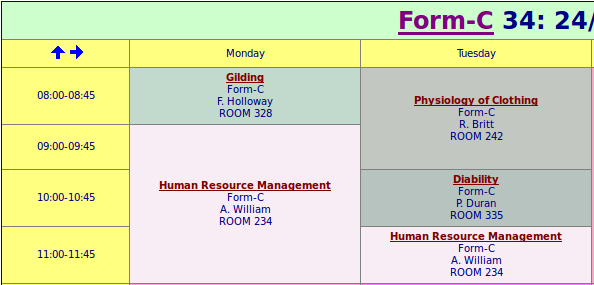
\includegraphics[width=0.8\textwidth]{../Billeder/MimosaSoftware.png}
	\caption{Udsnit af Mimosa Scheduling Software\cite{mimosaPicture}}
	\label{fig:Mimosa}
\end{figure}
\FloatBarrier
Et andet stykke software, ved navn Mimosa Scheduling Software\cite{Mimosa}, (se figur \ref{fig:Mimosa}), fokuserer mere på de grundlæggende udfordringer såsom overbooking og at gøre det nemmere at kunne ændre på skemaerne, hvis der skulle opstå en uventet udfordring. Programmet er i stand til at lave skemaer for lærere, elever, klasser og lokaler; altså alt det som enhver dansk folkeskole har brug for. Institutionerne henter programmet, udarbejder deres egne ressourcer, dvs. lærere, elever, lokale mm. og fordeler derefter disse ud over dagene. Programmet vil så fortælle, om dette kan lade sig gøre, og hvis det ikke er tilfældet, vil det fortælle hvorfor\cite{MimosaTutorial}. I modsætning til School Master Scheduling er Mimosas program mere henvendt til skemalæggerne og ikke så meget til de studerende. 

Begge programmer løser dog så at sige ikke selve skemalægningsopgaven, da dette stadig gøres manuelt af skemalæggeren eller de individuelle studerende for deres eget skema, men fungerer i stedet som et kontrollerende led. Ser man på de 10 mest anbefalede skemalægningsprogrammer fra hjemmesiden TopTenReviews\cite{top10Schedulers}, er de ikke rangeret ud fra automatisk skemalægning. Programmet som kommer tættest på, vil være Auto-Scheduler, men denne funktionalitet virker kun for medarbejdere ud fra en historik og er derfor ikke automatisk skemalægning. Besøger man et af de ti anmeldte programmers hjemmesider, finder man ingen information omkring programmernes evner indenfor dette. Et program som vil være i stand til helt automatisk at lave skemaer til alle på for eksempel en dansk folkeskole, udelukkende ud fra information om de ansatte, eleverne og tilgængelige klasselokaler, vil derfor være innovativt og nyttigt. Disse top-ti skemalægningsværktøjer er også mest henvendt til firmaer, så firmaerne kan tildele hver lønmodtager arbejdsopgaver og holde styr på, hvor meget løn hver lønmodtager får, hvilket er noget anmeldelsesiden går meget op i og bedømmer skemalægningsværktøjerne ud fra.

\subsubsection{Tabulex}
\begin{figure}[h!]
	\centering
	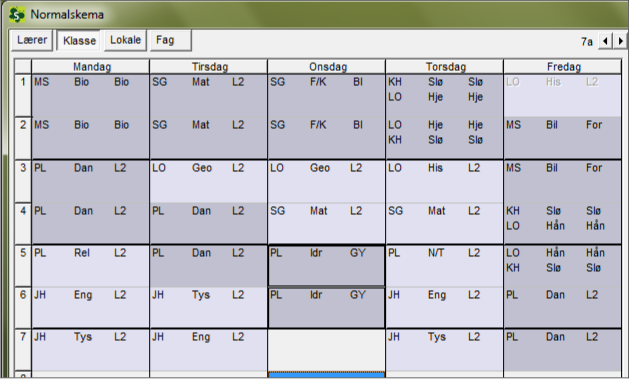
\includegraphics[width=0.8\textwidth]{../Billeder/TabulexPicture.png}
	\caption{Tabulex skemalægningsprogram\cite{Tabulex}}
	\label{fig:TabulexPicture}
\end{figure}
\FloatBarrier
På Tingstrup skole vil et program ved navn Tabulex (se figur \ref{fig:TabulexPicture}) blive taget i brug i forbindelse med skemalægningen. Det er et skemalægningsværktøj, der som de forrige kræver, at brugeren stiller programmet en hel del krav, heriblandt hvordan lærerens tid skal prioriteres, hvornår lektionerne lægges, og hvor meget hver af disse regler skal prioriteres og overholdes af programmet\cite{Tabulex}. Tabulex kan selv forsøge i bedste fald at lægge et skema ud fra de mange begrænsninger, som skemalæggeren har stillet, og undervejs vil programmet informere brugeren, hvis kravene som er opstillet ikke muliggør et skema, og man kan rette dem til. Herefter er det  muligt at fortsætte skemalægningen eller starte lægningen forfra. Ligesom de andre skemalægningsværktøjer, kommer det med en grafisk brugerflade, som understøtter drag\&drop, og som er rimeligt overskuelig. Tabulex kan dog ikke holde styr på regnskabet ligesom værktøjerne i forhenværende afsnit, men dette er heller ikke hvad programmet er lavet til at håndtere. Det bør nævnes, at Tabulex har en dybdegående dokumentation omkring hvordan programmet eksporterer til en CSV-fil\cite{Tabulex_csv}, og da et af kravene stillet af vores case er, at det endelige skema skal kunne inddrages i SkoleIntra, KMD Elev og andre programmer\cite{interview_Kaerby}, som netop tager imod CSV-formatet (se figur \ref{fig:kompatibleFiltyper}), er dette noget, vi vil kigge nærmere på.
\begin{figure}[h!]
	\centering
	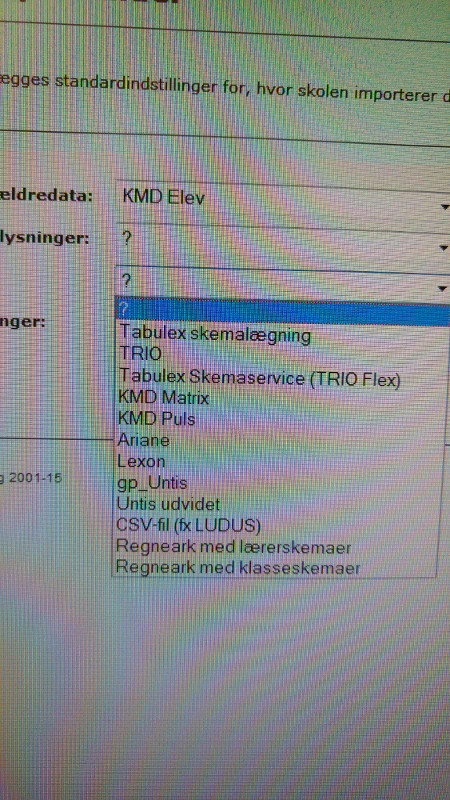
\includegraphics[width=0.4\textwidth]{../Billeder/Skemaimportering_filtyper_Intra.jpg}
	\caption{Skolens online system SkoleIntra kan læse forskellige filformater}
	\label{fig:kompatibleFiltyper}
\end{figure}
\FloatBarrier
\subsubsection{KMD Educa}
Et andet program Tingstrup-skolen bruger er KMD Educa, hvilket er en samling af forskellige værktøjer\cite{KMD}, der gør det muligt blandt andet at vikarføre, lægge skemaer og håndtere karakterresultater for den enkelte elev, som går på skolen eller har gået på skolen. Dette er en af de mange grunde til, at Aalborg Kommune har valgt at benytte sig af KMD Educa programmet ``Elev''\cite{useCase_KMD_Educa_Elev}.

\subsubsection{Docendo}
Vores case, Kærbyskolen, brugte et program ved navn Docendo før skolestart 2015, men selvom firmaet selv giver udtryk for, at deres program er meget fleksibelt\cite{Docendo}, var det ikke fleksibelt nok for skolen, og de valgte derfor i stedet at lægge skemaet manuelt. Programmet tillader at lægge skemaet elektronisk, lave varierende lektionslængder og tælle brugte timer, så eleverne hverken får for få lektioner eller for mange. Ud fra deres video\cite{Docendo_video}, er det nemt at gå til; klasserne kan holdes styr på i en grafisk brugerflade og lektionerne kan flyttes rundt som man nu lyster. Hvis man gør dette, ændres tidspunktet i lektionsrubrikken også. Skemaet lægges dog for hver uge, men dette er i sidste ende ligegyldigt, da den tidligere uges skema godt kan genbruges.

\subsubsection{Untis}
Untis er et af de mest anvendte skemalægningsprogrammer i Europa. Untis skriver, at deres program kan bruges af alle og har funktionerne til at gøre skemalægningen nem og overskuelig for skemalæggeren. Nogle af fordelene ved Untis er programmets fuldautomatiske skemaoptimering med en hurtig optimeringsalgoritme, samt at det er egnet til alle skoletyper.\cite{UntisDK}
Untis har et brugervenligt system, hvor man indtaster skolens specifikke oplysninger, og ud fra oplysningerne kan Untis danne et skema til skolen baseret på skolens krav og fokus - eksempelvis om der må være det samme fag to dage i træk. På figur \ref{fig:untisskema} ses det, at Untis har et fleksibelt skemalægningssystem, hvor der kan ændres i flere variabler baseret på skolens interesser. 
\begin{figure}[h!]
	\centering
	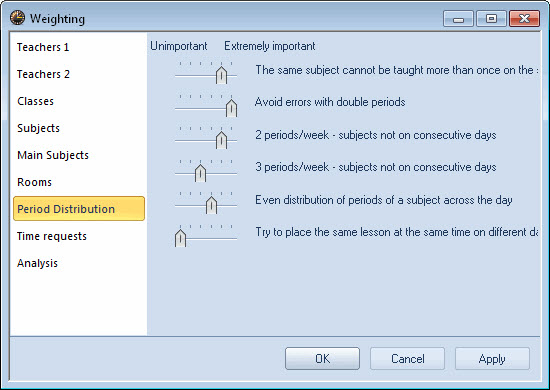
\includegraphics[width=0.8\textwidth]{../Billeder/untisskema.jpg}
	\captionsource{Untis' fleksible skemalægningssystem}{\url{http://www.school-timetabling.com/}}
	\label{fig:untisskema}
\end{figure}
\FloatBarrier
Algoritmen, som Untis bruger, giver flere resultater, hvor man selv kan bestemme, om skemaet passer til ens behov. Når skemaet er blevet lagt, er der flere muligheder for, hvordan det kan blive vist frem.\cite{UntisInt}

\subsubsection{Brute Force}
Vi vil nu undersøge nogle af de teknologier, som et program kunne benytte sig af for at finde frem til et skema. Den mest systematiske løsning, og måske den løsning der er nemmest af gå til, er brute force-metoden. Brute force går som navnet antyder ud på at bruge rå kraft for at finde løsningen. Måden dette gøres på i en computer, er ved at prøve samtlige muligheder, indtil man når det ønskede resultat.

I forhold til skemalægning, ville man altså forsøge samtlige sammensætninger af moduler i løbet af ugen, for alle klasse. For at undersøge om dette ville virke, kan vi regne ud hvor mange skemaer et program maksimalt ville skulle teste.

$$ (\text{UgentligeModuler})! \times \text{AntalKlasser} = \text{AntalSkemaer}$$

Hvis vi indsætter informationer fra Kærbyskolen som har 12 klasser og 10 lektioner om dagen får vi følgende antal skemaer:
$$ (10\cdot 5)! \cdot 12 = 3,65\cdot 10^{65} $$

Som det kan ses ud fra det enorme tal vi lige har regnet ud, er det umuligt at tjekke samtlige skemaer, for at finde det bedste, og man må derfor nøjes med at finde de første $n$ skemaer ved hjælp af bruteforce. Da man som regel kun ændrer \'en ting af gangen når man brute-forcer, kunne disse $n$ skemaer dog komme til at ligne hinanden meget, og man får ikke stor variation i skemaet.

\subsubsection{Heuristisk metode}
Ordet heuristisk bliver i ordbogen defineret som ``vedr. erkendelse af ny viden, opnået fx ved systematisk søgning efter information eller afprøvning af muligheder''\cite{Ordnet}.

\subsubsection{Monte Carlo / Las Vegas}

\subsubsection{Genetiske algoritmer}


	\subsection{Brugerovervejelser}
Da dette projekt handler om at udvikle et system til at hjælpe skolerne med deres skemalægning, nytter det ikke noget at lave et system, de ikke kan gennemskue, og dermed bruge. Derfor er det relevant at kigge på brugernes færdigheder i forhold til at benytte informationssystemer.

På figur \ref{fig:docendo_skema} er skemalægningsprogrammet Docendo vist. Dette program blev tidligere brugt på Kærbyskolen og som det ses af figuren, bruges drag\&drop-princippet til at indsætte moduler i skemaet. Dette gør programmet meget intuitivt og let at bruge, noget som Kærbyskolen efterspørger. I interviewet med Kærbyskolen fortalte skemalæggeren, at programmet skulle være meget let at bruge for, at det var en god løsning for skolen.

\begin{figure}[h!]
	\centering
	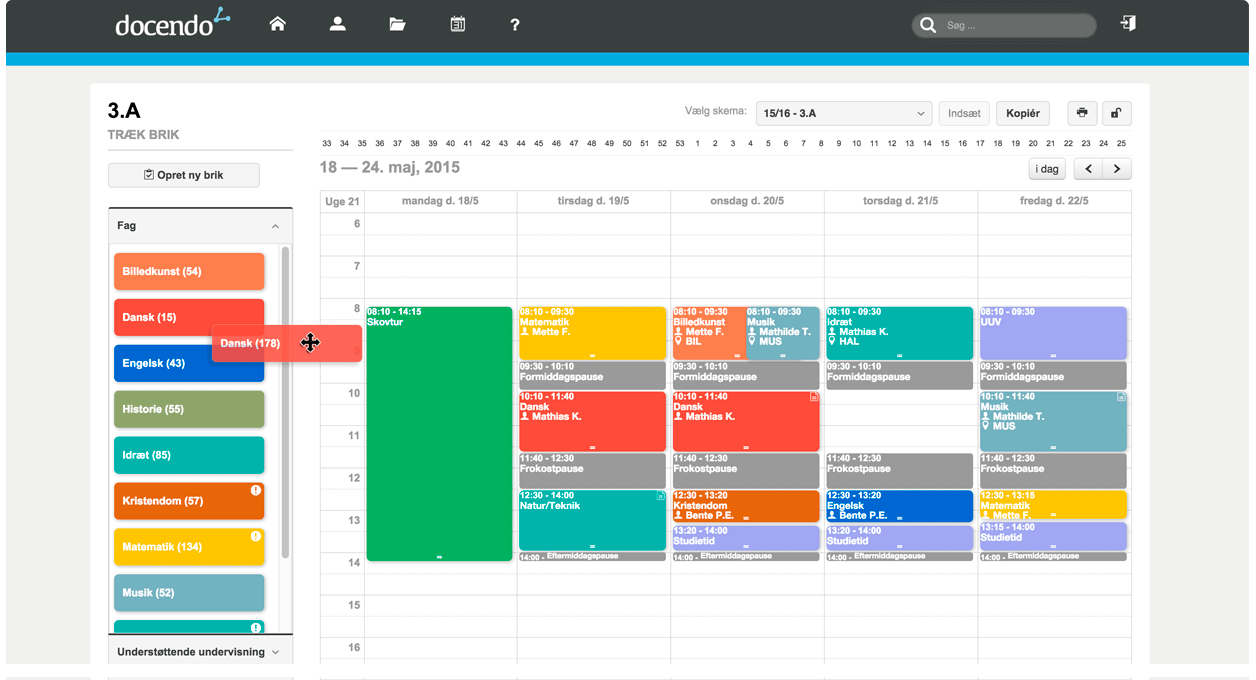
\includegraphics[width=\textwidth]{Docendo}
	\captionsource{Docendos skemalægningsprogram}{\url{https://docendo.dk/folkeskole.html}}
	\label{fig:docendo_skema}
\end{figure}

På skoler er der flere forskellige systemer der skal arbejde sammen for, at alt fungerer. Skemaet skal eksempelvis lægges ind på nettet i SkoleIntra, så eleverne kan få adgang til det. Derfor er det vigtigt, at et eventuelt program der laves til at hjælpe med denne skemalægning er kompatibelt med disse allerede eksisterende programmer, så der ikke skal manuelt arbejde til at konvertere filer fra det ene system til det andet. Heldigvis bruges der i de fleste programmer CSV-filer, hvilket er tekstfiler med kommaseparerede værdier, som så kan læses af de respektive programmer. Det der gør denne filtype nem at arbejde med, er, at vi ved at udskrive informationer omkring skemaet i forskellige rækkefølger, men i samme filformat, kan eksportere til alle disse programmer.

Ved at lave en måde at eksportere på til de forskellige formater, kan skemaet tages direkte fra vores program, og sættes ind i de andre programmer. Dette betyder for skolen at programmet potentielt kun skal bruge informationer omkring skolen og lærere, og så kan den selv lave et skema, der er klar til, at de kan bruge det direkte.

Interviewet med Tingstrup skole fortalte, at det ikke var nødvendigt med en decideret grafisk brugerflade, så længe at der var noget som fortalte brugeren, hvad programmet lavede. Det vil sige, at det ikke er nødvendigt at have flot grafik, så længe brugeren kan se programmets status. 

Dermed er kravet fra de to skoler et system, som ikke behøves at have en grafisk brugerflade, men skal være nemt at bruge, samtidig med at det hele tiden skal oplyse om, hvor langt det er, så brugeren (skemalæggeren) kan se, om systemet er gået i stå, eller om der er opstået problemer. Når programmet skal laves, er det altså vigtigt, det holdes for øje, at brugerne af systemet ikke nødvendigvis ved hvad de skal, og at programmet derfor skal guide dem igennem processen med at indtaste data.
	\subsection{SWOT-analyse}
For at forstå \school bedre, kan vi lave en SWOT-analyse af skolen som en virksomhed. En SWOT-analyse er en model man kan benytte for at analysere et firmas Styrker, Svagheder, Muligheder og Trusler (Strengths, Weaknesses, Opportunities, Threats), heraf navnet. På denne måde ønsker vi at forstå mere om skolens virkemåde, samt se hvor vi med et program kan forbedre skolens muligheder.

\subsubsection*{Styrker}
I form af Kærbyskolens mindre størrelse på kun 335 elever og 33 lærere \cite{Kaerbyskolens-laerere}, er der muligheder for et tættere arbejde mellem de ansatte. Dette kom eksempelvis til udtryk, under skemalægningen hvor alle lærere og pædagoger arbejde sammen om at lægge et skema.

Selvom det ifølge skolen selv ikke var den største succes at lægge skemaet på denne måde, viser det alligevel hvilket tæt samarbejde de ansatte kan have med hinanden på skolen.

For skolen giver dette tætte samarbejde en højere kvalitet, da man ved at snakke med alle parter, sikrer sig at alle behov på skolen bliver hørt. Hvis vi igen tager udgangspunkt i den fælles skemalægning, betød samarbejdet at alle lærere og dermed alle klassetrin blev repræsenteret under skemalægningen, og at skemaerne derfor blev gode for samtlige klasser på skolen. 

\subsubsection*{Svagheder}
Ved skolens nuværende model for skemalægningen, er der nogle svagheder. Der er lagt timer af i lærernes skema til at de kan træde ind som vikar for andre lærere. På grund af skemaerne, er deres forberedelsestid meget splittet op, hvilket gør at lærerene bliver stresset hvis de skal nå at forberede sig til at være vikar, samtidig med at de også skal undervise deres egne klasser.

Så selvom der er aflagt timer i skemaet til at de kan være vikarer, vælger skolen som regel at bruge eksterne vikarer, af hensyn til lærerende på skolen. Dette er en svaghed, som kunne afhjælpes ved at skemaet blev lagt anderledes.

\subsubsection*{Muligheder}
[Ikke skrevet endnu]

\subsubsection*{Trusler}
Kærbyskolen har ikke lokaler nok på skolen, til alle dennes fag. Det vil sige at lokaler til fag som idræt, musik og sløjd bliver lånt andetsteds fra. Skolen låner lokaler fra institutionen Kulturskolen, og skolen opnår dermed faciliteter til at undervise i disse fag. Denne afhængighed af Kulturskolen skaber dog nogle udfordringer og trusler mod Kærbyskolen. Lokalerne på kulturskolen er ikke altid ledige, og når skemaerne skal lægges, skal der tages højde for dette. 

Måden hvorpå skemalæggeren tog højde for dette, var ved at sætte nogle faste intervaller hvor hver klasse havde mulighed for at bruge lokalerne. Dette satte nogle store begrænsninger i forhold til skemalægninger, hvor man nu mistede megen frihed i forhold til placeringen af timerne, på grund af kravene til at låne lokaler. Til det møde hvor alle de ansatte i fællesskab skulle ligge skemaer, kom skemalæggeren med en række ufærdige skemaer hvorpå disse intervaller var lagt ind, og ud fra dette skulle de så fylde resten af skemaet op. 
	\section{Problemafgrænsning}
	
I vores problemafgrænsning ønsker vi at indsnævre det problem, som tages med fra problemanalysen og finde frem til de fokusområder, som vi finder vigtigst inden for skemalægning i folkeskoler og ønsker at tage udgangspunkt i under problemløsningen. Prolemafgrænsningen skulle altså gerne hjælpe med at finde frem til en god problemformulering. Det vil i afsnittet altså blive beskrevet, hvilke fokusområder der til- og fravælges.

For at sikre et projekt, som har relevans i vores tid og for vores specifikke case, tages der udgangspunkt i vores case, Kærbyskolen, og kun \school da vi grundet tidspres, ikke har tid til at inkludere flere cases samtidig med at sikre vores løsning er kompatibel under begge skolers skemalægningsprocedure og publiceringen af disse.

\subsection*{Pædagogisk læring}
På Kærbyskolen har skemaer, som tager deres udgangspunkt i pædagogisk læring og elevtrivsel, i år været højt prioriteret. Dette kom til udtryk under interviewet med skolen, hvor det blev beskrevet, at pædagogiske overvejelser i forhold til skemalægning blev diskuteret meget og var noget, som nuværende løsninger i følge skolen ikke forholder sig nok til. Vi ønsker derfor at lægge fokus på skemalægning med vægt på pædagogisk overvejelser.

\subsubsection*{Brugergrænseflade}
Brugergrænseflade fravælges som fokusområde og dette gøres hovedsageligt grundet projektets omfang og tidsbegrænsning. Dette betyder dog ikke, at brugervenlighed glemmes helt. Kærbyskolen lagde under det foretagede interview vægt på, at programmer skal være nemme at bruge, og at det er vigtigt, at programmet løbende giver brugeren en status. Dette ønsker vi så at tage hensyn til i så stort et omfang, som muligt.

\subsubsection*{Andre afgrænsninger}
I forbindelse med overvejelser omkring projektets omfang og de opstillede tidsbegrænsninger, som vi må forholde os til, har vi desuden måtte gøre os nogle andre fravalg af fokuspunkter. Dette er valg som vi føler er nødvendige for, at projektet realistisk kan gennemføres i tide og samtidig ikke rammer den egentlige kvalitet af problemløsningen eller programfunktionalitet, men blot gør det endelige program lidt mindre.

Vi har med valget af Kærbyskolen som case fravalgt at tage højde for valgfag, da skolen kun går til 6. klasse, hvor disse endnu ikke findes. 

Vores case, Kærbyskolen, er en meget lille skole og derfor har de ikke mulighed for at have alle fagene på skolens grund. Kærbyskolen er nødt til at arbejde sammen med andre parter for at opfylde kraverne om idræts- og hjemkundsskabsfaciliteter. Vi har dog valgt, at fokuset ikke skal være lagt på lokalerne, men på pædagogisk læring og brugerflade.

Vi fokuserer på skemalægning på Kærbyskolen, men ønsker ikke at tage højde for skolens såkaldte J-klasser for autismediagnostiserede elever, da der dannes skemaer efter elevens individuelle behov. Derfor vil vi fokusere på at lægge skema til klasserne 0 til 6.

%\subsubsection*{Valgfag}
%Vi har fravalgt valgfag, som et fokusemne, da vi har valgt at arbejde ud fra en case, hvor skolen i dette tilfælde går op til 6. klasse, hvor de ikke har valgfag.

%\subsubsection*{Lokaler}
%Vores case, Kærbyskolen, er en meget lille skole og derfor  har de ikke mulighed for at have alle fagene på skolensgrund. Kærbyskolen er nødt til at arbejde sammen med andre parter for at opfylde kraverne om idræts og hjemkundsskabs faciliteter. Vi har dog valgt, at fokuset ikke skal være lagt på lokalerne, men på pædagogisk læring og brugerflade.

%Vi fokuserer på skemalægning på Kærbyskolen, men ønsker ikke at tage højde for skolens såkaldte J-klasser for autismediagnostiserede elever, da der dannes skemaer efter elevens individuelle behov. Derfor vil vi fokusere på at lægge skema til klasserne 0 til 6.

    \section{Problemformulering}
    På baggrund af de observationer og erfaringer, der er blevet gjort gennem rapportens problemanalyse, er problemet i afsnit \ref{afg} blevet afgrænset, og vi er kommet nærmere det, som vi mener er kernen i vores problemstilling om skemalægning i danske folkeskoler. Vi er nået frem til, at det der er behov for på folkeskoler ikke blot er en nemmere, hurtigere form for skemalægning, men også en skemalægning, som har fokus på pædagogiske overvejelser. Dette har givet os nedenstående problemformulering.

``Hvordan hjælper man, ved hjælp af software, skemalæggeren med at lægge vægt på pædagogiske overvejelser under skemalægingen?''
    \newpage
    
	\bibliographystyle{apa}
	\bibliography{sources}

    \section{Bilag}
    \begin{enumerate}
	\item Hvad er jeres nuværende procedure angående skemalægning?

	Som regelt bølger det op og ned mellem teams og ledelsen, i år er det alle teams der har arbejdet sammen. De startede med at snakke om hvilke områder de ville prioritere, og så arbejde de ud fra disse områder. De forsøgt i år at tage udgangspunkt i pædagogiske principper, dog har det været meget svært at gøre, grundet begrænsninger som f.eks. lokalemangel. I år har de inddelt lærerne i teams for de forskellige klassetrin. 0 klasse har sit eget team, og ellers er teamsene: 1-2 årgang, 3-4 og 5-6 årgang. Lærerne har så kun undervist i de klasser deres team håndtere (med meget få undtagelser).

	Ud fra deres oplevelser med skemalægningen i år har de fundet ud af, at ikke alle lærere skal være med til at lægge skemaet, samt at det er svært at indarbejde pædagogiske overvejelser og værdier i skemaet. Næste år vil de udpege ledere for hvert team, og så skal lederne arbejde sammen om at lave skemaet, så der bliver færre mennesker involveret.

	Selvom det var svært at ligge skemaerne i år, har måden de gjorde det på ført til gode samtaler mellem lærer og elever, for at afdække alles ønsker.

	Måden de gjorde det på sidste år var, at lærere hver især skrev en række ønsker, og gav dem til \'en person som derefter skulle udarbejde skemaet på baggrund af alle disse ønsker. Det havde dog ført til at lærernes forberedelsestid blev spredt ud over hele dagen, hvilket nogle lærere havde været utilfredse med. F.eks. kunne deres skema lyde: 45 minutters undervisning, 45 minutters pause, 90 minutters undervisning og så 45 minutters forberedelse. Lærerne ønskede på baggrund af dette at de mindst skulle have 60 minutters forberedelse af gangen, da det gav den bedste mulighed for at forberede sig ordentligt til timerne.

	Nogle lærerer var ansat på skolen, på 2/3 af den normale arbejdstid, der skulle i skemaet tages højde for dette, på en sådan måde at deres timer ikke overlappede med deres arbejde på andre institutioner.

\noindent\makebox[\linewidth]{\rule{\paperwidth}{0.4pt}}

	Helt team, anderledes i år. Normalt bølger det op og ned mellem teamet  og ledelsen. Så i år har teamene fået det. Så de har snakket hvad de ville prio og hvordan man så har kunne arbejde derfra. forsøgt at tage udgangspunkt i pedagoiske præncipper, dog har det været meget svært, låst af nogen ting som fx. mangle på idræts faciliteter, sløjt og hjemkunskabs lokaler. Skolen havde så i år forsøgt på noget andet.. at i år har de valgt at fordele lærene i 3teams  1-2, 3-4 og 5-6. inden for de klasser har du så også teams for fx 5 og 6. dog har lærene både haft timer for 5 og 6 klasse. De er blevet kloggere, de har fundet ud af at ikke hele teamet der skal ligge det. det var meget svært i forsøg med også at have pedagoiske karakteristiker og værdier, svært at lave efter det. Næste år vil de prøve det samme, dog med en form leder indenfor teamet, så lederne til sidst vil gå sammen om det. Måden de gjorde det i år har ikke virket så godt. Har givet en del reflektioner, der har ført til en masse snakken med eleverene og lærene. Før i tiden fik de massere af ønsker ind. kunne en person sætte det ind i et program, hvorefter de så vile forsøge. Sidste år stort problem med ikke sammensat forberedningstid. fx 45 undervisning, 45 pause, 90 time, 45 forberedelse fx. Vigtigt for dem er mere end 1 times forberedelse af gangen, da de fik mere ud af at kunne forberede sig i længere tid af gangen i stedet for en masse gange med kort tid. Dog er det også vigtigt at det passer med børnene. 

	De har også kombi ansatte, dvs. nogen der måske kun er 2/3 ansat på skolen, så skemaet skulle også passe med at disse kombi ansatte ikke havde noget andet arbejde sammentidigt et andet sted.

\noindent\makebox[\linewidth]{\rule{\paperwidth}{0.4pt}}
	
	\item Hvor lang tid bruger I på at lave skemaer? (før og efter reform?)

	I år tog det meget lang tid, da de var 60 ansatte om det. Der var på forhånd bestemt nogle få ting, såsom at 1. klasse skulle have billedkunst om mandagen, men alle de små detaljer og præcise tidspunkter skulle der opnås enighed om. Planen var oprindeligt at det skulle tage 3-4 timer at nå frem til det skema, reelt tog det dog omkring 8 timer, for de 60 mennesker. 

	Tanken var også oprindeligt at der i løbet af et år skulle være 4 skemaer. Grundet at det tog så lang tid at lægge skemaet, og at det var et meget stort arbejde, er der ingen der har taget initiativ til at der skulle lægges et nyt, da der var gået 1/4 af skoleåret. Derfor bliver der enten kun 2 skemaer i løbet af året, eller i værste fald kun dette ene.

	Skolen har eksperimenteret med fagdage, altså hvor en hel dag var sat af til et enkelt fag. Erfaringerne fra dette var dog at det førte til meget spildtid, og at lærerene blev meget frustreret over det.

	Til at holde styr på timer, har de brugt Microsoft Excel.
	\noindent\makebox[\linewidth]{\rule{\paperwidth}{0.4pt}}
	
	Det har taget lang tid i år. De tog teamsne ind, hvorfra der i forvegen var delt lokaler ud til folk. fx 1 klasse har billedkunst mandag. Originalt tænkt 3-4 timer. brugt 3 gange så meget, hvor hele personalet var i gang. fx var der 8-9 igang. dvs de har cirka være 60 mand og cirka 8 timer. Og de fandt som sagt ud af at det ikke var alle der skullle have alle med i skemalægningen. Man kan finde ud af at noget ikke fungere. original tanke var 4 skema perioder. dog er det fx ikke blevet ændret. Fagdage har de også prøvet lidt med. fx dansk hver 3 tirsdag. De brugte for meget tid. og personalet blev meget fustreret over det. De brugte tidligere et program kaldet: Dosendo? Dosindo? Dusindo? Dosindu? 

Har brugt regneark i forsøg på at beregne timemængde osv..

Største problem virker til at være 
Tror ikke man vil kunne tage højde for alt, så ville være fornuftingt hvis %nooo
	\noindent\makebox[\linewidth]{\rule{\paperwidth}{0.4pt}}
	
	\item Bruger skolen faste skemaer eller ugentlige?
	Skolen har som regel 4 skemaer på et år, hvor hver skoledag er inddelt i moduler på 30 minutters længde.

	\noindent\makebox[\linewidth]{\rule{\paperwidth}{0.4pt}}
	4 gange om året cirka
	kører haltimers moduler 
	\noindent\makebox[\linewidth]{\rule{\paperwidth}{0.4pt}}

	\item Hvor tit skal der ændres i skemaer?

	Hvis der er noget i skemaet der ikke fungere, bliver der lavet små ændringer for at få det til at fungere, men ellers kun de 4 skemaer om året (som dog ikke er blevet gjort i år).

	\noindent\makebox[\linewidth]{\rule{\paperwidth}{0.4pt}}
	De har ændret lidt af tingene på skemaet i starten, da de kunne se at nogen ting ikke fungerede. De havde originalt plan om at ændre skemaet, så de ville have 4 forskellige skemaer i løbet af året. Men allerede nu kan man se at det ikke vil ske, da det skulle have været ændret, men det blev det ikke. 
	\noindent\makebox[\linewidth]{\rule{\paperwidth}{0.4pt}}

	\item Findes buffer-timer? 

	Der findes på skolen ingen ``buffer-timer''. Dette betyder at der ikke må ske aflysninger af timer, men at der i stedet skal sættes en vikar på.

	\noindent\makebox[\linewidth]{\rule{\paperwidth}{0.4pt}}
	Ingen bufertimer. vikar... aldrig aflysninger
	\noindent\makebox[\linewidth]{\rule{\paperwidth}{0.4pt}}
	

	\item Er lektiecafe på skemaet? Skal der være en lærer til stede (en lærer pr klasse)?

	Der er lektiecaf\'e på skemaet. Der er lærere til hver klasse. Det vil sige at lektiecaf\'en virker helt som et normalt fag. Dog kan der godt være flere lærere til et fag, så de kan have lærere der dækker hvert fagområde. Lektecaf\'en har de lagt sidst på dagen, da dette fungerer bedst i forhold til hvilke lokaler der er til rådighed på kulturskolen, hvor de låner lokaler.

	\noindent\makebox[\linewidth]{\rule{\paperwidth}{0.4pt}}
	Er der. Har de slåset med, pga kulturskole osv. det skal forældre give tilladelse til... lektiecafe lagt sidst på dagen pga binding fra kulturskolen.  

	Lærer per klasse i dette. De er administreret som et fag , så den samme lærer på bestemte lærere. For 5-6 klasse 3-4 lærerer så man kan gå ind i et bestemt "fags" lokale. 
	\noindent\makebox[\linewidth]{\rule{\paperwidth}{0.4pt}}
	
	\item Er der faste lærer til hver klasse? Hvor længe beholder man samme lærer?

	Ja. Lærene underviser i deres årgangs teams. dvs de underviser for 2 årgange om året. altså hvis man var på 1-2 klasses teamet underviste man 1-2 klasse.
	
	\item Hvordan håndterer i lokaler? (f.eks. ved store klasser?, hvad hvis 2 skal være i fysik-lokalet? Faste lokaler?)
	
	Bruger flex skema. Binder af lokaler pga. kulturskole
	
	\item Hvordan håndterer I lærernes tid på skolen? (i form af forberedelsestid)
	
	Et skema skal kunne understøtte læring og trivsel, eller sammenhængende blokke, så man vil kunne nå at fordybe sig. Det ville være dejligt at kunne tage højde for små ting i skemalægningen, frem for at sige om hver ting at enten vægter det, eller også gør det ikke. Altså kunne det have været rart at kunne sige hvor meget hver enkelt parameter betyder for skemaet. 
	
	\item Hvor mange timer om året pr lærer? pr elev? (Har skolen data?)
	
	Vil kunne måske få skoledata
	
	\item Hvilket system bruger I til håndtering eller udarbejdning af skemaer?

	I år brugte de håndkraft, klippeklister osv \ldots De plejede dog at lave det med et program. Dosendo? Dosindo? Dusindo? Dosindu? 
	
	\item Hvordan samarbejder det med andre systemer? Kan du importere andre filer?
	
	Skal kunne arbejde med SkoleIntra (det kan det system de brugte før) Der er dog en ny platform på vej, minuddanelse. ville kunne være dejligt hvis det skal kunne arbejde sammen med det. Ville være oplagt hvis det kunne samarbejde med et regneark. Når de var rigtigt mange var det dejligt at de havde det visuelt overblik, altså en grafisk fremstilling af skemaet, især når de arbejder i teams
	
	\item Fremvisning af programmet?
	
	Kan ikke da de ikke har noget. Viste dog SkoleIntra siden som de bruger. så forældre, elever og lærer kan fx se skemaet online osv\ldots 
	
	\item Vikarhåndtering, bliver det sat ind i systemet?
	
	Det bliver sat ind i skemaet. de er blevet sat ind i SkoleIntra, hvor man så ville kunne se det. Opgaverne er blevet givet til teamsne, hvor de har x timer til at være vikar. så hvis der er mangel på nogen så kan en anden tage over\ldots taget fra forberedelse, hvor de har lidt for mange timer i forvejen med det. Dog har de en presset hverdag, hvilket gør at de sætter ekstern vikar på. Meget vigtigt at kunne være komfortabel(?) med. 
	
	\item Bliver en vikartime regnet som en normal time? (uddannelsesniveauet er jo ikke det samme)
	
	Ja.
	
	\item Komfortabel med at arbejde i CLI?
	
	Fortrækker noget meget nemt visuelt, drag\&drop, lige nu er de nødt lærerne er nødt til at komme ind til Jesper, hvorefter han så skal ændre det.
	
	\item Prioritering af fag efter tid på dagen?
	
	Der er intet fastsat fra ledelsen, men teamsne har snakket om det. Der har været snak om at mindske sværhedsgraden i de sene timer (14-15), hvor eleverne er ved at være trætte. De har haft mange diskussioner om hvordan det er bedst at håndtere den bevægelse som skal være i løbet af dagen. Der har været snak om at lave det som et fast modul fra 10 til 11, hver dag. Der har dog været en del bindinger i forhold til lokalerne, da det ikke er sikker at idrætslokalet er frit.
	
	\noindent\makebox[\linewidth]{\rule{\paperwidth}{0.4pt}}
	Ikke nogen overvejelse fra ledelsen.. har været på teamsne .. har et bud på at de nok er bredt ud, så det ikke er. Der har også været snak om sværheden af undervisning ved fx 14-15. De har haft en del debater om bevægelse, om man skulle være firkantet, have det som et bond ( fx fra 10-11 )  så de lavet noget aktivt ændten før eller efter pause... Dette er blevet gjort på mange forskellige måder, da de som sagt har brugt en masse teams.. De har været låst med tidspunkter hvor de kunne have fx idræt pga. binding fra kulturskolen. Jo ældre de er, jo flere bindinger.  dvs. næste år vil de starte med 5-6 klasse osv. de har kunne snakke om brug af lokaler med andre teams. pedagoer mere med i skemaerne. men skal stadig have sammenhængdene dage, hvor pedagoerne sf. også skal være med i det fritids efter skolen. plotter selv skemaerne de har lavet ind i intra... hvorefter de så kan sætte skemabrikker på... man skal lave "brikker" for at kunne sætte et fag ind... dog virker det ikke til at man kan slette gamle brikker (Jesper viste ikke)
	programmet kan tage regneark Det er vist en del af it's learning. 

	Syntes opgaven var vigtig for lærene, da det var dem der skulle kunne udholde skemaet i noget tid. Og man skal nok ikke starte på bar bund. 
	\noindent\makebox[\linewidth]{\rule{\paperwidth}{0.4pt}}
	\item Prioritering af læreres ønsker?

	Da skemaet blev lavet i teams af personalet, så lærene selv skulle tage holdning for hvad de ønskede at prioritere.  
	
\end{enumerate}
    \subsection{Interview med Tingstrup Skole}
\label{InterviewTingstrup}
\begin{enumerate}
	\item Hvad er jeres nuværende procedure angående skemalægning?
	
	1 Viseskoleleder, 1 afdelingsleder og leder ligger grundskemaet. Viseskolederen laver finpudsningen.
	grundskemaet: Det, som gælder fra skoleårets start.
	\item Hvor lang tid bruger I på at lave skemaer? (før og efter reform?)
	
	Efter: ca. 8 arbejdsdage for alle ledere. ca. 3 dage på seminar og ca. 3 dage efter eleverne har fået ferie. Ved ikke om de hjælper hinanden eller om de bare kommer med inputs. Starter klokken 8, nogle gange først hjemme klokken ca. 22:00.
	\item Bruger skolen faste skemaer eller ugentlige?
	
	Alle elever har 2 skemaer. Et som kører fra sommerferie til jul, og et som kører fra jul til sommerferien.
	\item Hvor tit skal der ændres i skemaer?
	
	Hvis der er noget som ikke fungerer, hvis en lærer er længerevarende syg, eller hvis en lærer finder et andet arbejde, bliver der ændret i skemaet.
	\item Findes buffer-timer? 
	
	Nej. Hvis en dansk-lærer er syg, kan en anden lærer godt komme ind, og så lave undervisningen om. For eksempel, dansk læreren er syg, og så kommer en matematiklærer og overtager timen, og laver dansktimen om til matematik.
	\item Hvordan håndterer man timer der ikke finder sted?
	
	Hvis en lærer ikke er tilstede, kommer der en vikar på. Dette kan både være lærer, eller vikar.
	\item Er lektiecafe på skemaet? Skal der være en lærer til stede (en lærer pr. klasse)?
	
	Efter 1. August blev lektiecaf\'een obligatorisk, så den er på skemaet. Nogle gange ligger den først på dagen, andre dage ligger den sidst på dagen.
	En lærer skal være til stede på lektiecaféen. Lektiecaféen hedder faglig fordybelse. 7, 8, og 9. består af 12 klasser, og 12 lærer, og dette ligger samtidig. Ud af de 12 lærer kan en engelsk, en dansk og en matematik, så de kan de forskellige ting som eleverne har brug for hjælp til, og så må eleverne selv vælge hvilken faglig fordybelses time de går til. Har de brug for hjælp til Engelsk, kan de gå til Engelsk timen den ene dag, og den næste matematik, hvis dette er tilfældet.
	
	Der findes et stillerum, hvor eleverne kan gå hen og skrive hvad de skal i fred og ro. Der er en lærer til stede, som sørger for der er stille i dette rum.
	Det fungere dog kun sådan i overbygningen. I indskolingen og mellemklassen har hver lærer, hver deres klasse, som klassen skal være ved. De vælger ikke selv.
	Det hedder faglig fordybelse i alle klasser bortset fra 9. klasse, hvor det hedder lektiecafé. Dette kan muligvis skyldes at de selv vælger, hvilken ``café'' de går til.
	\item Er der faste lærer til hver klasse? Hvor længe beholder man samme lærer?
	
	Faste lærere.
	0 klasse kører for sig selv.
	Nye lærer fra 1. klasse, som fortsætter gennem hele indskolingen 1-3.
	Nye lærere igen fra 4-6 klasse, også klasselæreren. De flytter også klasselokalet.
	Nye lærere igen fra 7-9 klasse, også klasselæreren. De flytter også klasselokalet. I 7. klasse bliver der rykket sammen fra flere skoler, og der bliver dermed lavet nye klasser. De flytter klasselokaler igen i 9. klasse, da der er et området som er blevet renoveret, og som kun er tilegnet 9. klasser. Her sker der også af og til at klasserne har tværfaglige forløb, hvor to klasser går sammen og arbejder.
	\item Hvordan håndterer i lokaler? (f.eks. ved store klasser?, hvad hvis 2 skal være i fysik-lokalet? Faste lokaler?)
	
	I idræt har hele årgangen idræt samtidig. Ellers sørges der for at de andre lokaler sådan som madkundskab- og fysik-lokalerne, kun bliver lagt til rådighed for 1 klasse i et bestemt modul.
	\item Hvordan håndterer I lærernes tid på skolen? (i form af forberedelsestid)
	
	Lærernes på fuld tid har mødetid 7:30, og nogle dage har de længere dage end andre. Nogle dage møder de 7:30, og har fri klokken 17, da det er her, de har mødetid. Eleverne har fri klokken 15, så her er der møde fra 15:00 til 17:00. Altid møde om Tirsdagen, da det er her, lærerne er på skolen til 17. Lærerne arbejder ikke hele dagen, og den resterende tid, bruger de på ``andet'', hvilket bliver brugt til andet så som forberedelse, ringe til forældre, eller møder.
	\item Hvor mange timer om året pr. lærer? pr. elev? (Har skolen data?)
	
	Lærerne arbejder ca. 40 timer om ugen, og de arbejder 42 uger om året.
	
	0-3 går i skole fra 8 til 14:00 hver dag
	
	4-6 går i skole fra 8 til 14:20 hver dag.
	
	7-9 går i skole fra 8 til 15:05 hver dag.
	\item Hvilket system bruger I til håndtering eller udarbejdning af skemaer?
	
	De bruger KMD Educa Personale, kaldet Puls før sommerferien. Skemaprogrammet de bruger til at lave skemaerne i, hedder tabulex, et program de endnu ikke har brugt. Det program de brugte tidligere, hed Matrix.
	Skemaerne bliver lagt over i KMD Educa Personale, hvor der også bliver lavet vikardækning og hvor der bliver tjekket efter om de har mødetid anderledes. Hvis en lærer har haft klassemøde til klokken 20:00, har de arbejdet 3 timer for meget, og de kan derfor gå ind og ændre i skemaet så de møder senere eller går hjem tidligere, hvis de ikke har undervisning, og kun hvis de syntes de har udført deres arbejde. Lærerne kan derfor selv håndtere deres flex-tid. De kan også se hvor meget de har at bruge af.
	\item Hvordan samarbejder det med andre systemer? Kan du importere andre filer?
	
	Skemaerne importeres ind i KMD Educa Personale når det er færdigt fra Tabulex / Matrix, og fra kan der trykkes på en knap, som så bliver ført over til Intra, hvor alle andre kan se det. Smårettelser bliver lavet i Educa Personale.
	KMD Educa Personale har selv et skemalægningsprogram, som dog ikke er helt færdig endnu, og for svært at lægge skemaer i.
	\item Vikarhåndtering, bliver det sat ind i systemet?
	
	Vikardækning laves i Educa Personale, og så bliver det eksporteret til Intra, så lærere og vikarer kan se det.
	\item Bliver en vikartime regnet som en normal time? (uddannelsesniveauet er jo ikke det samme)
	
	En vikar får højere løn, da en læreres løn allerede ligger i deres løn, hvor en vikar skal forberede sig ud over.
	\item Komfortabel med at arbejde i CLI?
	
	Der skal være en grafisk brugerflade. Personligt er hun ligeglad med om det er en CLI eller en GUI, så længe man kan se der sker noget med det samme.
	\item Prioritering af fag efter tid på dagen?
	
	Det kan ikke lade sig gøre, så der bliver ikke prioriteret på sådan noget som fysik og idræt.
	Dog bliver der sørget for der ikke kun ligger kreative fag på samme dag (gælder dog ikke for overbygningen, da de har disse fag som valgfag), ligesom der heller ikke kun ligger de boglige på en dag.
	\item Prioritering af læreres ønsker?
	
	Lærerne laver en ønskeliste inden skemalægningen, hvor de blandt andet kan ønske efter at undervise i bestemte klassetrin og hvilke tidspunkter de helst vil undervise. Lærerne bestemmer fuldstændig selv, hvad de skriver på denne ønskeliste, og så kan skemalæggerne forsøge at gøre deres bedste på at opfylde så mange ønsker som muligt
\end{enumerate}
    \newpage
    \begin{landscape}
\subsection{Timetabel}
\label{TimetalsKrav}
\begin{table}[h!]
	\centering
	\resizebox{25cm}{!}{%
		\begin{tabular}{lllllllllllll}
			Timetal (minimumstimetal og vejledende timetal) for fagene &                               &     &     &     &     &     &     &     &     &     &     &                         \\
			Klassetrin                                                 &                               & Bh. & 1.  & 2.  & 3.  & 4.  & 5.  & 6.  & 7.  & 8.  & 9.  & Timetal i alt           \\
			\textbf{A. Humanistiske fag}                               &                               &     &     &     &     &     &     &     &     &     &     &                         \\
			Dansk                                                      & \textit{(minimumstimetal)}    &     & 330 & 300 & 270 & 210 & 210 & 210 & 210 & 210 & 210 & 2.160                   \\
			Engelsk                                                    & \textit{(vejledende timetal)} &     & 30  & 30  & 60  & 60  & 90  & 90  & 90  & 90  & 90  & 630                     \\
			Tysk eller fransk                                          & \textit{(vejledende timetal)} &     &     &     &     &     & 30  & 60  & 90  & 90  & 90  & 360                     \\
			Historie                                                   & \textit{(minimumstimetal)}    &     &     &     & 30  & 60  & 60  & 60  & 60  & 60  & 30  & 360                     \\
			Kristendomskundskab                                        & \textit{(vejledende timetal)} &     & 60  & 30  & 30  & 30  & 30  & 60  &     & 30  & 30  & 300                     \\
			Samfundsfag                                                & \textit{(vejledende timetal)} &     &     &     &     &     &     &     &     & 60  & 60  & 120                     \\
			\textbf{B. Naturfag}                                       & \textit{}                     &     &     &     &     &     &     &     &     &     &     &                         \\
			Matematik                                                  & \textit{(minimumstimetal)}    &     & 150 & 150 & 150 & 150 & 150 & 150 & 150 & 150 & 150 & 1.350                   \\
			Natur/teknik                                               & \textit{(vejledende timetal)} &     & 30  & 60  & 60  & 90  & 60  & 60  &     &     &     & 360                     \\
			Geografi                                                   & \textit{(vejledende timetal)} &     &     &     &     &     &     &     & 60  & 30  & 30  & 120                     \\
			Biologi                                                    & \textit{(vejledende timetal)} &     &     &     &     &     &     &     & 60  & 60  & 30  & 150                     \\
			Fysik/kemi                                                 & \textit{(vejledende timetal)} &     &     &     &     &     &     &     & 60  & 60  & 90  & 210                     \\
			&                               &     &     &     &     &     &     &     &     &     &     &                         \\
			\textbf{C. Praktiske/musiske fag}                          &                               &     &     &     &     &     &     &     &     &     &     &                         \\
			Idræt                                                      & \textit{(vejledende timetal)} &     & 60  & 60  & 60  & 90  & 90  & 90  & 60  & 60  & 60  & 630                     \\
			Musik                                                      & \textit{(vejledende timetal)} &     & 60  & 60  & 60  & 60  & 60  & 30  &     &     &     & 330                     \\
			Billedkunst                                                & \textit{(vejledende timetal)} &     & 30  & 60  & 60  & 60  & 30  &     &     &     &     & 240                     \\
			Håndværk og design samt madkundskab                        & \textit{(vejledende timetal)} &     &     &     &     & 90  & 120 & 120 & 60  &     &     & 390                     \\
			\textbf{D. Valgfag}                                        & \textit{(vejledende timetal)} &     &     &     &     &     &     &     & 60  & 60  & 60  & 180                     \\
			\textbf{E. Årligt minimumstimetal pr. klassetrin}          &                               & 600 & 750 & 750 & 780 & 900 & 930 & 930 & 960 & 960 & 930 & 7.890 ekskl. bh. /8.490
		\end{tabular}
	}
	\caption{Viser hvor mange timer hver årgang skal have af et fag\cite{Lovgivning}\\Note: Timetallene er angivet i klokketimer og uden pauser.Note: Bh.: Børnehaveklasse.}
\end{table}

\end{landscape}
\end{document}